\documentclass[letterpaper]{article}
\usepackage[margin=1in]{geometry}
\usepackage[utf8]{inputenc}
\usepackage{textcomp}
\usepackage{amssymb}
\usepackage{natbib}
\usepackage{graphicx}
\usepackage{gensymb}
\usepackage{amsthm, amsmath, mathtools}
\usepackage[dvipsnames]{xcolor}
\usepackage{enumerate}
\usepackage{mdframed}
\usepackage[most]{tcolorbox}
\usepackage{csquotes}
% https://tex.stackexchange.com/questions/13506/how-to-continue-the-framed-text-box-on-multiple-pages

\tcbuselibrary{theorems}

\newcommand{\R}{\mathbb{R}}
\newcommand{\Z}{\mathbb{Z}}
\newcommand{\N}{\mathbb{N}}
\newcommand{\Q}{\mathbb{Q}}
\newcommand{\C}{\mathbb{C}}
\newcommand{\code}[1]{\texttt{#1}}
\newcommand{\mdiamond}{$\diamondsuit$}
\newcommand{\PowerSet}{\mathcal{P}}
\newcommand{\Mod}[1]{\ (\mathrm{mod}\ #1)}
\DeclareMathOperator{\lcm}{lcm}

%\newtheorem*{theorem}{Theorem}
%\newtheorem*{definition}{Definition}
%\newtheorem*{corollary}{Corollary}
%\newtheorem*{lemma}{Lemma}
\newtheorem*{proposition}{Proposition}


\newtcbtheorem[number within=section]{theorem}{Theorem}
{colback=green!5,colframe=green!35!black,fonttitle=\bfseries}{th}

\newtcbtheorem[number within=section]{definition}{Definition}
{colback=blue!5,colframe=blue!35!black,fonttitle=\bfseries}{def}

\newtcbtheorem[number within=section]{corollary}{Corollary}
{colback=yellow!5,colframe=yellow!35!black,fonttitle=\bfseries}{cor}

\newtcbtheorem[number within=section]{lemma}{Lemma}
{colback=red!5,colframe=red!35!black,fonttitle=\bfseries}{lem}

\newtcbtheorem[number within=section]{example}{Example}
{colback=white!5,colframe=white!35!black,fonttitle=\bfseries}{def}

\newtcbtheorem[number within=section]{note}{Important Note}{
        enhanced,
        sharp corners,
        attach boxed title to top left={
            xshift=-1mm,
            yshift=-5mm,
            yshifttext=-1mm
        },
        top=1.5em,
        colback=white,
        colframe=black,
        fonttitle=\bfseries,
        boxed title style={
            sharp corners,
            size=small,
            colback=red!75!black,
            colframe=red!75!black,
        } 
    }{impnote}
\usepackage[utf8]{inputenc}
\usepackage[english]{babel}
\usepackage{fancyhdr}
\usepackage[hidelinks]{hyperref}

\pagestyle{fancy}
\fancyhf{}
\rhead{CSE 101}
\chead{Monday, January 24, 2022}
\lhead{Lecture 9}
\rfoot{\thepage}

\setlength{\parindent}{0pt}

\begin{document}

\section{Priority Queue Implementations}
We will go through some prioriy queue implementations. 

\subsection{Unsorted List}
Store $n$ elements in an unsorted list. 

\bigskip 

\underline{Operations:}
\begin{itemize}
    \item \code{Insert}: $\BigO(1)$.
    \item \code{DecreaseKey}: $\BigO(1)$.
    \item \code{DecreaseMin}: $\BigO(1)$.
\end{itemize}
For Dijkstra, we would have $\BigO(|V|^2 + |E|)$. 

\subsection{Binary Heap}
Store elements in a balanced binary tree with each element having smaller key value than its children.

\begin{center}
    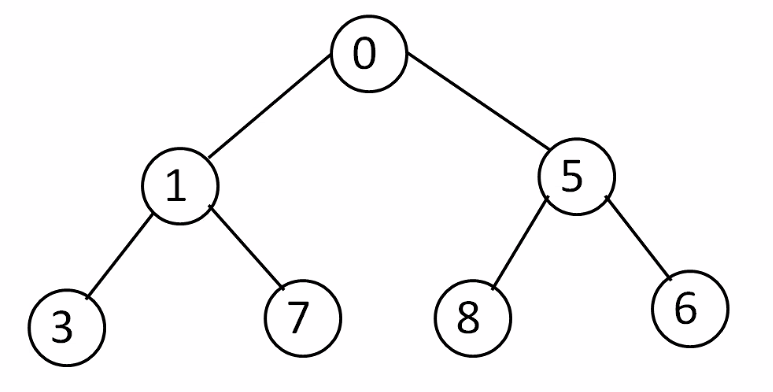
\includegraphics[scale=0.5]{../assets/bin_heap.png}

    \textbf{Figure: A binary heap.}
\end{center}
The smallest key is at the top (\code{0}) and there are $\log{n}$ levels. 

\bigskip 

\underline{Operations:}
\begin{itemize}
    \item \code{Insert}: Add the key at the bottom, then bubble the new key up until it's in the right place. This is done in $\BigO(\log(n))$ time. 
    \item \code{DecreaseKey}: We need to change the key. Then, we might need to bubble up the changed key until it's in the right place. This is done in $\BigO(\log(n))$ time. 
    \item \code{DecreaseMin}: We remove and then return the root node. Then, we move the bottom-most node to the root. After this, we might need to continuously bubble down the root node until it's in the right place. This is done in $\BigO(\log(n))$ time. 
\end{itemize}
For Dijkstra, we would have $\BigO(\log(|V|)(|V| + |E|))$. 


\subsection{d-ary Heap}
This is like a binary heap, but each node has $d$ children. 
\begin{center}
    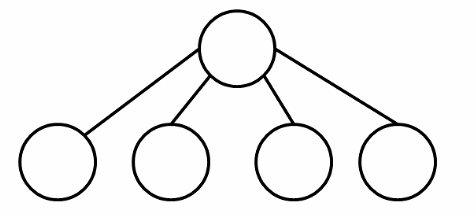
\includegraphics[scale=0.5]{../assets/dary_heap.png}

    \textbf{Figure: A 4-ary heap.}
\end{center}

There are $\log(n) / \log(d)$ levels, so bubble up is faster. However, bubble down is slower since we need to compare more children. 

\bigskip 

\underline{Operations:}
\begin{itemize}
    \item \code{Insert}: This is done in $\BigO(\log(n) / \log(d))$ time. 
    \item \code{DecreaseKey}: This is done in $\BigO(\log(n) / \log(d))$ time. 
    \item \code{DecreaseMin}: This is done in $\BigO(d\log(n) / \log(d))$ time. This is because, for bubble down, we need to consider the $d$ children. 
\end{itemize}
For Dijkstra, we would have $\BigO\left(\frac{\log(|V|)(d|V| +|E|)}{\log(d)}\right)$. 


\subsection{Fibonacci Heap}
This is an advanced data structure that uses amortization\footnote{So, you might spend more time on a particular operation, but the overall runtime will be ``consistent.''}. 

\bigskip 

\underline{Operations:}
\begin{itemize}
    \item \code{Insert}: This is done in $\BigO(1)$ time. 
    \item \code{DecreaseKey}: This is done in $\BigO(1)$ time. 
    \item \code{DecreaseMin}: This is done in $\BigO(\log(n))$ time. This is because, for bubble down, we need to consider the $d$ children. 
\end{itemize}
For Dijkstra, we would have $\BigO(|V|\log(|V|) + |E|)$. 

\section{Negative Edge Weights}
So far, we've talked about non-negative lengths. However, depending on what we're representing as lengths, we might have \emph{negative} lengths. That being said, the problem statement is the same - find the path with the smallest sum of edge weight. 

\bigskip 

Right now, Dijkstra's algorithm doesn't actually work on negative edge values. 

\subsection{Negative Weight Cycle}
\begin{definition}{}{}
    A \textbf{negative weight cycle} is a cycle where the total weight of edges is negative. 
\end{definition}
\textbf{Remarks:}
\begin{itemize}
    \item If $G$ has a negative weight cycle, then there are probably no shortest paths since we can go around the cycle over and over again. 
    \item For an undirected graph $G$, a single negative weight edge gives a negative weight cycle by going back and forth on it. So, we usually don't talk about the negative edge weight in the context of an undirected graph. 
\end{itemize}


\end{document}